\section{Assignment Problems}

\begin{frame}{Assignment Problems}
    \begin{itemize}[<+->]
        \item Students $s \in S$
        \item Rooms $r \in R$
        \item $r_s \in R$
        \item $n = |R| = |S|$
    \end{itemize}
\end{frame}

\subsubsection{House Allocation Problem}

\begin{frame}{House Allocation Problem}
\begin{itemize}[<+->]
    \item no initial assignments
    \item core property % Any allocation in the core of an economy is also Pareto optimal.
    \item pareto optimality 
    \item strategy proofness
\end{itemize}    
\end{frame}

\begin{frame}{Serial dictatorship (SD)}
    \textbf{Input:} Priority order $\pi$ of $n$ students and their respective preference reports. \\
    \textbf{We define:} \\
    $s_k := \pi(k)$, is the $k$'th agent \\
    $R_k$ is set of rooms left in $k$'th iteration \\
    $X_s(R)$ is student $s$ most preferred room out of $R$ \\
    \textbf{Algorithm:} 
    \begin{itemize}
    \item Iterate through $\pi$
    \item for $1 \leq k \leq n$: $r_{s_k} = X_{s_k}(R_k)$
    \end{itemize} 
    \begin{itemize}[<+->]
        \item Time complexity: $O(n)$
        \item Strategy proof and Pareto optimal
    \end{itemize}
\end{frame}

\begin{frame}{Random Serial dictatorship (RSD)}
    \textbf{Input:} $n$ students preference reports. \\
    \textbf{Algorithm:} 
    \begin{itemize}
    \item Create a random priority order $\pi$ (uniform distribution)
    \item run serial dictatorship mechanism on it
    \item Time complexity: $O(n)$ ($n = |S|)$
    \item strategy proof, ex-post pareto optimal, anonymous
\end{itemize} 
\end{frame}

\subsubsection{Housing Markets Problem}
\begin{frame}{Housing Markets Problem}
    \begin{itemize}
    \item participants have initial assignments
    \item core property % Any allocation in the core of an economy is also Pareto optimal.
    \item pareto optimality 
    \item strategy proofness
    \item <2->Why not just collect all items, and run RSD?
\end{itemize}    
\end{frame}

% ttc1
\begin{frame}{Top Trading Cycles (TTC)}
    \centering
    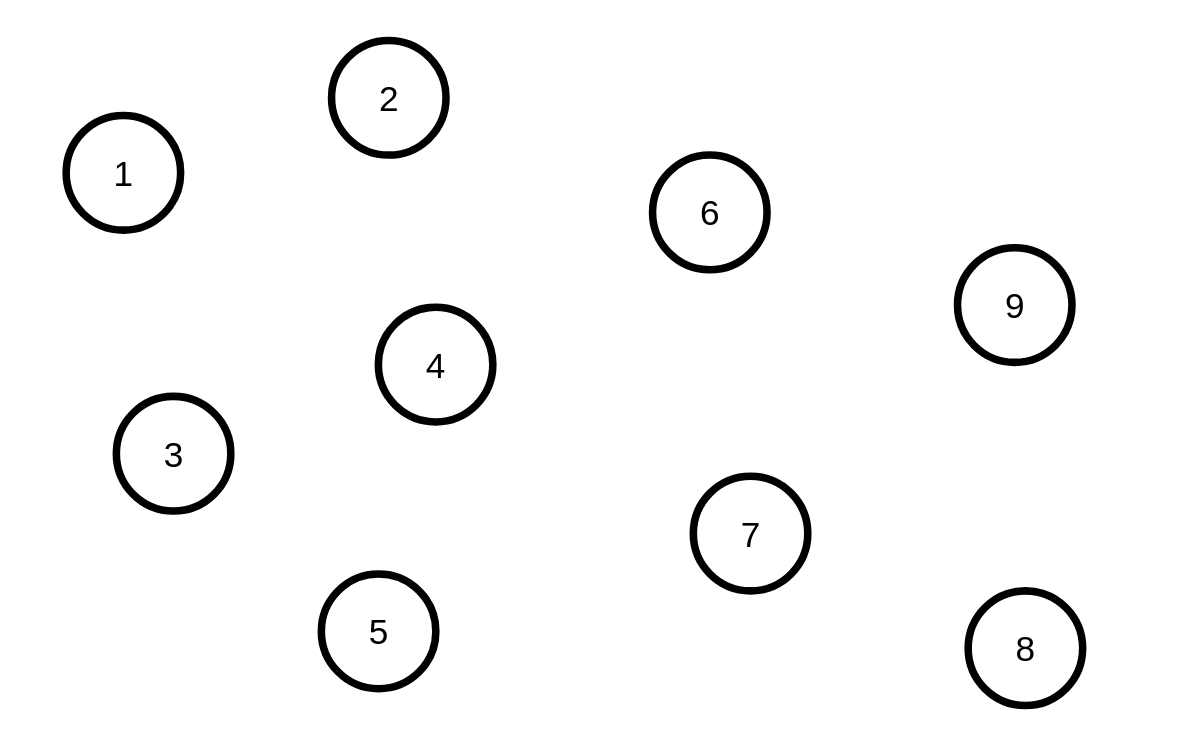
\includegraphics[width=10cm]{img/ttc/ttc1.png}
\end{frame}
% ttc2
\begin{frame}{Top Trading Cycles (TTC)}
    \begin{itemize}
    \item <2-> $S_1 = \{1,2,3,4,5\}$
    \end{itemize}    
    \centering
    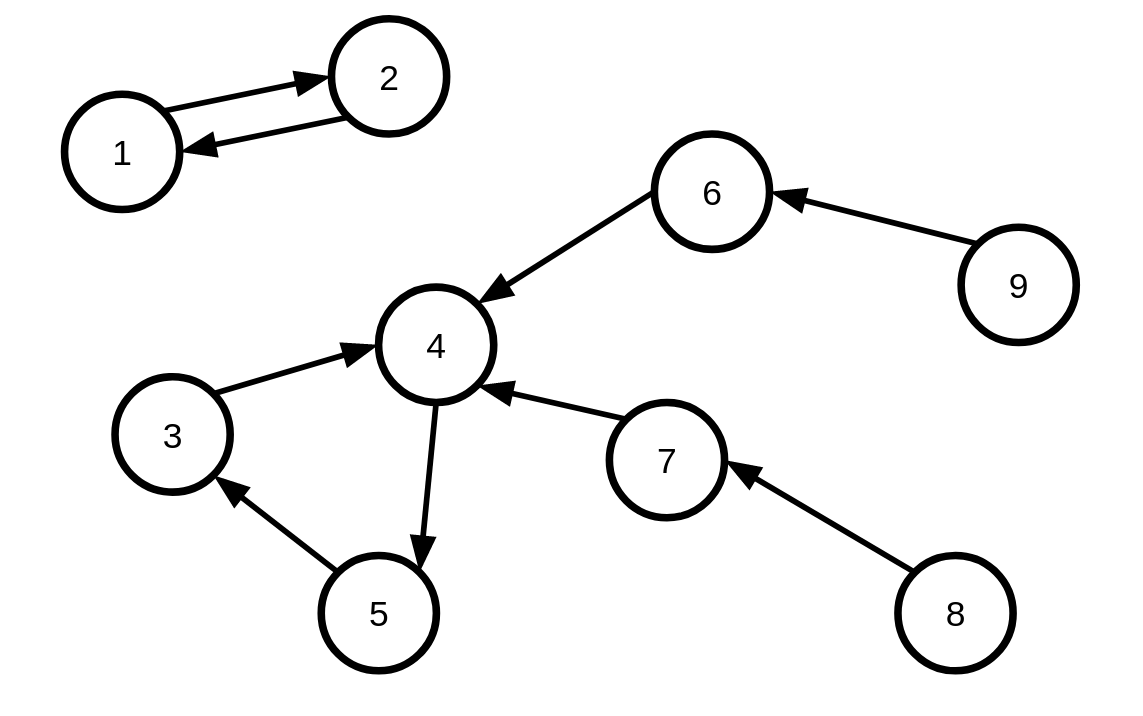
\includegraphics[width=10cm]{img/ttc/ttc2.png}
\end{frame}
% ttc3
\begin{frame}{Top Trading Cycles (TTC)}
    \begin{itemize}
    \item $S_1 = \{1,2,3,4,5\}$
    \item <2-> $S_2 = \{6\}$
    \end{itemize}   
    \centering
    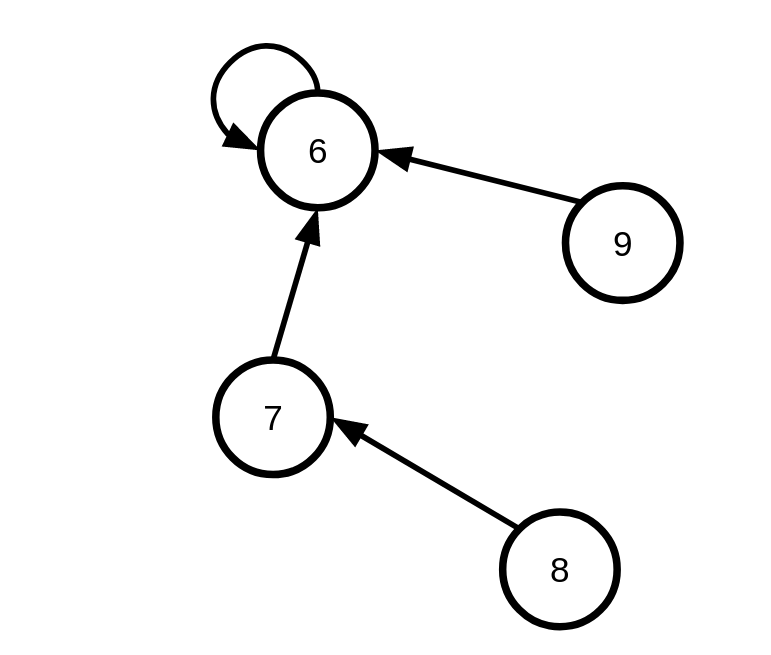
\includegraphics[width=9cm]{img/ttc/ttc3.png}
\end{frame}
%ttc4
\begin{frame}{Top Trading Cycles (TTC)}
    \begin{itemize}
    \item $S_1 = \{1,2,3,4,5\}$
    \item $S_2 = \{6\}$
    \item <2-> $S_3 = \{7,8\}$
    \end{itemize}   
    \centering
    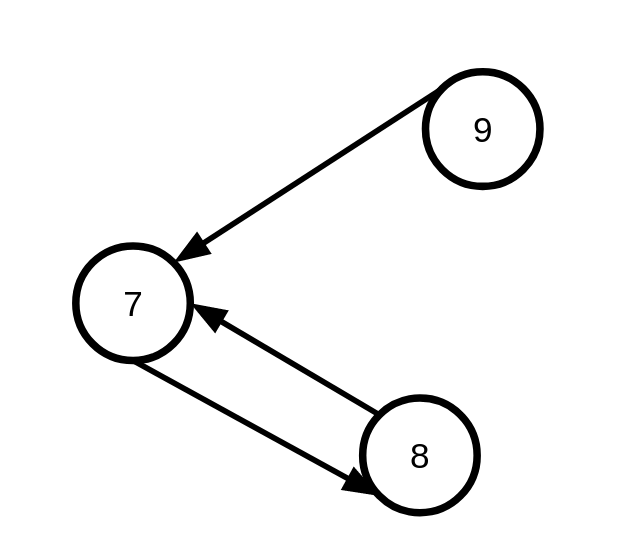
\includegraphics[width=8cm]{img/ttc/ttc4.png}
\end{frame}
%ttc5
\begin{frame}{Top Trading Cycles (TTC)}
    \begin{itemize}
    \item $S_1 = \{1,2,3,4,5\}$
    \item $S_2 = \{6\}$
    \item $S_3 = \{7,8\}$
    \item <2-> $S_4 = \{9\}$
    \end{itemize}  
    \centering
    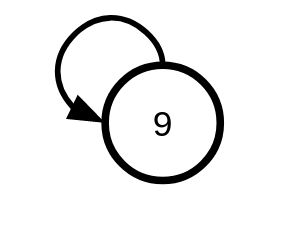
\includegraphics[width=3cm]{img/ttc/ttc5.png}
\end{frame}

\begin{frame}{Top Trading Cycles (TTC)}
    \begin{itemize}[<+->]
    \item Time complexity $O(n^2)$
    \item At least one cycle per round
    \item no node is part of more than one cycle
    \end{itemize}    
\end{frame}

\begin{frame}{Top Trading Cycles (TTC)}
    \centering
    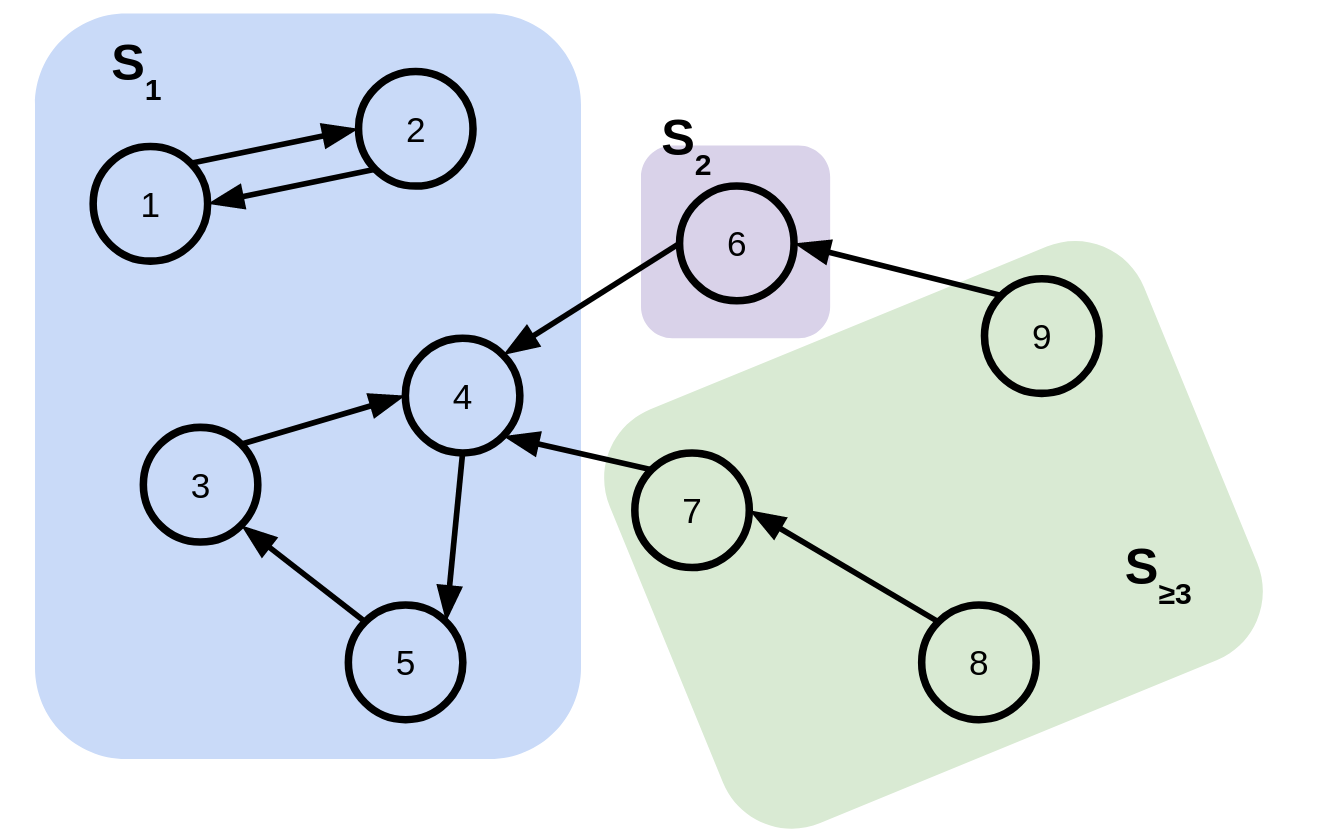
\includegraphics[width=12cm]{img/ttc/ttcstages.png}
\end{frame}

\subsubsection{RSD and TTC}
\begin{frame}{RSD and TTC}
    \begin{itemize}[<+->]
        \item RSD seems rudimentary
        \item Model house allocation problem with TTC by randomizing initial assignments
        \item \textbf{Randomized TTC and RSD are the same lottery mechanism!} \\
        (A. Abdulkadiraglu and T. Sonmez)
    \end{itemize}
\end{frame}